\documentclass[11pt,a4paper]{article}
\usepackage[utf8]{inputenc}
\usepackage[T1]{fontenc}
\usepackage{lmodern}
\usepackage[french]{babel}
\usepackage[margin=2.3cm]{geometry}
\usepackage{amsmath,amssymb,amsthm,mathtools}
\usepackage{bm}
\usepackage{graphicx}
\usepackage{booktabs}
\usepackage{enumitem}
\usepackage[dvipsnames]{xcolor}
\usepackage[most]{tcolorbox}
\usepackage{listings}
\usepackage{hyperref}
\hypersetup{colorlinks=true,linkcolor=NavyBlue,urlcolor=NavyBlue,citecolor=NavyBlue}
\usepackage{fancyhdr}
\pagestyle{fancy}
\fancyhf{}
\lhead{\small Chapitre 2 -- Les moindres carrés ordinaires}
\rhead{\small Explications détaillées}
\cfoot{\thepage}
\setlength{\headheight}{14pt}
\setlength{\parskip}{0.45em}
\setlength{\parindent}{0pt}

% ---------- Notation ----------
\newcommand{\vy}{\mathbf{y}}
\newcommand{\vX}{\mathbf{X}}
\newcommand{\ve}{\mathbf{e}}
\newcommand{\vb}{\mathbf{b}}
\newcommand{\vx}{\mathbf{x}}
\newcommand{\vbeta}{\bm{\beta}}
\newcommand{\veps}{\bm{\epsilon}}
\newcommand{\vi}{\bm{\iota}}
\newcommand{\Mm}{\mathbf{M}}
\newcommand{\Pm}{\mathbf{P}}
\newcommand{\I}{\mathbf{I}}
\newcommand{\C}{\mathbf{C}}
\newcommand{\D}{\mathbf{D}}
\newcommand{\A}{\mathbf{A}}
\newcommand{\XtX}{\vX'\vX}
\newcommand{\XtXi}{(\vX'\vX)^{-1}}
\newcommand{\E}{\mathbb{E}}
\newcommand{\Var}{\operatorname{Var}}
\newcommand{\Cov}{\operatorname{Cov}}
\newcommand{\tr}{\operatorname{tr}}
\newcommand{\rg}{\operatorname{rang}}
\newcommand{\sumi}{\sum_{i=1}^{n}}

% ---------- Boîtes ----------
\newtcolorbox{intuition}[1][]{colback=Cerulean!6,colframe=Cerulean!70!black,fonttitle=\bfseries,title={Intuition},#1}
\newtcolorbox{resultat}[1][]{colback=ForestGreen!6,colframe=ForestGreen!70!black,fonttitle=\bfseries,title={À retenir},#1}
\newtcolorbox{attention}[1][]{colback=BrickRed!5,colframe=BrickRed!75!black,fonttitle=\bfseries,title={Attention / piège fréquent},#1}
\newtcolorbox{detail}[1][]{colback=gray!5,colframe=gray!60!black,fonttitle=\bfseries,title={Calcul détaillé},breakable,#1}
\newtcolorbox{histoire}[1][]{colback=Goldenrod!8,colframe=Goldenrod!70!black,fonttitle=\bfseries,title={Pour aller plus loin / histoire},breakable,#1}
\newtcolorbox{exemple}[1][]{colback=Orchid!5,colframe=Orchid!70!black,fonttitle=\bfseries,title={Exemple numérique},breakable,#1}

\lstset{basicstyle=\ttfamily\small,breaklines=true,frame=single,backgroundcolor=\color{gray!6},
  columns=fullflexible,keepspaces=true,showstringspaces=false,commentstyle=\color{ForestGreen},
  literate={é}{{\'e}}1 {è}{{\`e}}1 {à}{{\`a}}1 {ê}{{\^e}}1 {ç}{{\c{c}}}1 {É}{{\'E}}1 {ù}{{\`u}}1 {ô}{{\^o}}1 {î}{{\^i}}1}

\newtheorem*{theoreme}{Théorème}

\begin{document}

% ======================= PAGE DE TITRE =======================
\begin{titlepage}
\centering
\vspace*{2.5cm}
{\LARGE\bfseries Chapitre 2 : Les moindres carrés ordinaires\par}
\vspace{0.6cm}
{\Large Explications détaillées, intuitions, démonstrations pas à pas\\ et compléments de recherche\par}
\vspace{1.2cm}
{\large Guide d'étude accompagnant les notes de cours\\ (réf. : W. H. Greene, \emph{Econometric Analysis}, ch.~3, 4 et 15.5)\par}
\vspace{2cm}
\begin{tcolorbox}[colback=white,colframe=NavyBlue,width=0.85\textwidth,title=Ce que contient ce document]
\begin{itemize}[leftmargin=*]
\item Chaque équation du cours reprise et \textbf{expliquée ligne par ligne} (y compris les étapes « après manipulation » que les notes sautent).
\item Des \textbf{intuitions} géométriques et économiques, des \textbf{exemples numériques} calculés à la main.
\item Des \textbf{figures} et une \textbf{réplication de l'étude de Monte Carlo} du cours.
\item Des éléments \textbf{historiques} (Legendre, Gauss, Markov, Yule, Frisch, Waugh, Lovell\dots).
\item Une liste des \textbf{coquilles} relevées dans les notes, une \textbf{fiche de révision} et des \textbf{exercices corrigés}.
\end{itemize}
\end{tcolorbox}
\vfill
{\small Les numéros d'équation entre crochets, par ex. [13], renvoient aux équations des notes de cours.}
\end{titlepage}

\tableofcontents
\newpage

% ======================= 0. BOITE A OUTILS =======================
\section{Boîte à outils : l'algèbre matricielle dont on a besoin}

Tout le chapitre est écrit en notation matricielle. Avant de commencer, voici le strict nécessaire, avec la raison pour laquelle chaque outil sert.

\subsection{Dimensions et notation}
\begin{center}
\begin{tabular}{@{}lll@{}}
\toprule
Objet & Dimension & Signification \\
\midrule
$\vy$ & $n\times 1$ & les $n$ observations de la variable dépendante \\
$\vX$ & $n\times K$ & les $K$ variables explicatives (une colonne par variable, une ligne par individu) \\
$\vx_i$ & $K\times 1$ & la $i$-ème ligne de $\vX$, écrite en colonne ; donc $\vx_i'$ est la ligne $i$ \\
$\vbeta$ & $K\times 1$ & les vrais coefficients (inconnus, « population ») \\
$\veps$ & $n\times 1$ & les vraies erreurs (inconnues, non observées) \\
$\vb$ & $K\times 1$ & l'estimateur MCO de $\vbeta$ (calculé à partir des données) \\
$\ve$ & $n\times 1$ & les résidus MCO (calculés à partir des données) \\
\bottomrule
\end{tabular}
\end{center}

\textbf{Astuce de vérification :} dans un produit $\A\mathbf{B}$, le nombre de colonnes de $\A$ doit égaler le nombre de lignes de $\mathbf{B}$. Vérifier les dimensions permet de détecter la moitié des erreurs. Par exemple $\XtX$ est $(K\times n)(n\times K)=K\times K$ et $\vX'\vy$ est $(K\times n)(n\times 1)=K\times 1$.

\subsection{Transposée}
$(\A')'=\A$, \quad $(\A+\mathbf{B})'=\A'+\mathbf{B}'$, \quad $(\A\mathbf{B})'=\mathbf{B}'\A'$ (l'ordre s'inverse !).
Une matrice est \emph{symétrique} si $\A'=\A$. Exemple clé : $\XtX$ est toujours symétrique car $(\XtX)'=\vX'(\vX')'=\XtX$.

\subsection{Un scalaire est égal à sa transposée}
Si $a$ est un nombre ($1\times1$), alors $a'=a$. C'est l'astuce qui permet de passer de [7] à [8] : $\vb_0'\vX'\vy$ est $1\times 1$ et sa transposée est $\vy'\vX\vb_0$, donc les deux sont égaux.

\subsection{Rang et inverse}
Le \emph{rang} de $\vX$ est le nombre de colonnes linéairement indépendantes. $\vX$ est de \emph{plein rang (colonne)} si $\rg(\vX)=K$ : aucune variable n'est une combinaison linéaire exacte des autres. Dans ce cas, et seulement dans ce cas, $\XtX$ est inversible.

\begin{attention}
Exemples où le plein rang échoue (\emph{multicolinéarité parfaite}) :
\begin{itemize}[nosep]
\item inclure une constante \emph{et} une indicatrice pour chaque catégorie (homme \emph{et} femme) : « piège des variables indicatrices », car $\text{homme}+\text{femme}=1=$ constante ;
\item inclure l'âge, l'année de naissance et l'année d'observation (âge $=$ année $-$ naissance) ;
\item avoir moins d'observations que de variables ($n<K$).
\end{itemize}
Le logiciel (Stata, R) retire alors automatiquement une variable (« omitted because of collinearity » ou coefficient \texttt{NA}).
\end{attention}

\subsection{Matrice définie positive}
Une matrice symétrique $\A$ ($K\times K$) est \emph{définie positive} si $\mathbf{c}'\A\mathbf{c}>0$ pour tout vecteur $\mathbf{c}\neq \mathbf 0$, et \emph{semi-définie positive} si $\mathbf{c}'\A\mathbf{c}\ge 0$. C'est la généralisation matricielle de « nombre positif ».

Pourquoi $\XtX$ est définie positive quand $\vX$ est de plein rang :
\[
\mathbf{c}'\XtX\mathbf{c}=(\vX\mathbf{c})'(\vX\mathbf{c})=\|\vX\mathbf{c}\|^2=\sumi (\vx_i'\mathbf{c})^2\ \ge 0,
\]
et c'est nul seulement si $\vX\mathbf{c}=\mathbf 0$, ce qui (plein rang) n'arrive que si $\mathbf{c}=\mathbf 0$.

De même, pour n'importe quelle matrice $\D$, $\D\D'$ est semi-définie positive car $\mathbf{c}'\D\D'\mathbf{c}=\|\D'\mathbf{c}\|^2\ge0$ (sert pour Gauss-Markov).

\subsection{Trace}
La trace d'une matrice carrée est la somme de ses éléments diagonaux. Propriétés :
$\tr(\A+\mathbf{B})=\tr\A+\tr\mathbf{B}$, \ $\tr(c\A)=c\,\tr\A$, \ $\tr(\A\mathbf{B}\C)=\tr(\mathbf{B}\C\A)=\tr(\C\A\mathbf{B})$ (permutation circulaire), et pour un scalaire $a$, $\tr(a)=a$.
Elle sert pour estimer $\sigma^2$ (section~\ref{sec:sigma2}).

\subsection{Dérivées matricielles (règles [10] et [11])}
Le cours dit qu'il n'est pas nécessaire de connaître ces règles. Voici quand même pourquoi elles sont vraies, sur un exemple à $K=2$ : c'est rassurant.

Soit $\mathbf{a}=(a_1,a_2)'$ et $\vb=(b_1,b_2)'$. Alors $\mathbf a'\vb=a_1b_1+a_2b_2$ et
$\dfrac{\partial\, \mathbf a'\vb}{\partial\vb}=\begin{pmatrix}\partial/\partial b_1\\ \partial/\partial b_2\end{pmatrix}(a_1b_1+a_2b_2)=\begin{pmatrix}a_1\\a_2\end{pmatrix}=\mathbf a.$

Pour une forme quadratique avec $\A$ symétrique, $\vb'\A\vb=a_{11}b_1^2+2a_{12}b_1b_2+a_{22}b_2^2$, donc
\[
\frac{\partial\,\vb'\A\vb}{\partial\vb}=\begin{pmatrix}2a_{11}b_1+2a_{12}b_2\\2a_{12}b_1+2a_{22}b_2\end{pmatrix}=2\A\vb .
\]
\begin{resultat}
Ce sont exactement les analogues de $\frac{d}{db}(ab)=a$ et $\frac{d}{db}(ab^2)=2ab$ en dimension 1. Retenir l'analogie suffit.
\end{resultat}

% ======================= 1. INTRODUCTION =======================
\section{Le modèle de régression linéaire (Greene 3.1--3.2)}

\subsection{Le modèle [1]}
\[
y_i=\beta_1+\beta_2x_{i2}+\dots+\beta_Kx_{iK}+\epsilon_i=\vx_i'\vbeta+\epsilon_i,\qquad i=1,\dots,n.
\]
\begin{itemize}
\item $\vx_i=(1,x_{i2},\dots,x_{iK})'$ : le « 1 » en première position correspond à la constante $\beta_1$.
\item $\vx_i'\vbeta$ est la \emph{partie systématique} : sous l'hypothèse $\E[\epsilon_i\mid\vx_i]=0$, c'est l'espérance conditionnelle $\E[y_i\mid\vx_i]$, c'est-à-dire la valeur moyenne de $y$ chez les individus ayant les caractéristiques $\vx_i$.
\item $\epsilon_i$ regroupe tout ce qui influence $y_i$ mais n'est pas dans $\vx_i$ (facteurs omis, erreurs de mesure, hasard).
\end{itemize}
En empilant les $n$ équations : $\vy=\vX\vbeta+\veps$.

\begin{exemple}[title={Exemple économique}]
Équation de salaire (Mincer) : $\ln(\text{salaire}_i)=\beta_1+\beta_2\,\text{scolarité}_i+\beta_3\,\text{expérience}_i+\epsilon_i$. Ici $\beta_2$ est l'effet (en log, donc $\approx$ en \%) d'une année d'étude supplémentaire, \emph{à expérience donnée}. $\epsilon_i$ contient par exemple l'habileté, la motivation, la chance.
\end{exemple}

\subsection{Population contre échantillon : la distinction la plus importante du chapitre}
\begin{center}
\begin{tabular}{@{}lll@{}}
\toprule
& Population (inconnu) & Échantillon (calculé) \\
\midrule
Coefficients & $\vbeta$ & $\vb$ (ou un candidat quelconque $\vb_0$) \\
Termes aléatoires & erreurs $\epsilon_i=y_i-\vx_i'\vbeta$ & résidus $e_i=y_i-\vx_i'\vb$ \\
Partie systématique & $\E[y_i\mid\vx_i]=\vx_i'\vbeta$ & valeur prédite $\hat y_i=\vx_i'\vb$ \\
\bottomrule
\end{tabular}
\end{center}
L'équation [4], $y_i=\vx_i'\vbeta+\epsilon_i=\vx_i'\vb_0+e_i(\vb_0)$, dit simplement qu'on peut découper $y_i$ de deux façons : « vraie partie systématique + vraie erreur » (inobservable) ou « partie prédite + résidu » (observable). \textbf{Les résidus ne sont pas les erreurs} : ce sont leurs estimations.

\subsection{Pourquoi la notation $\vb_0$ ?}
$\vb_0$ désigne \emph{n'importe quel} vecteur candidat. À chaque candidat correspondent des résidus $e_i(\vb_0)$. Les MCO choisissent, parmi tous les candidats, celui qui rend les résidus « les plus petits » au sens de la somme des carrés ; ce gagnant est noté $\vb$ (sans indice).

% ======================= 2. DERIVATION =======================
\section{Le vecteur des coefficients MCO (Greene 3.2.1)}

\subsection{Le critère [5]--[6]}
\[
S(\vb_0)=\sumi e_i(\vb_0)^2=\sumi (y_i-\vx_i'\vb_0)^2=(\vy-\vX\vb_0)'(\vy-\vX\vb_0).
\]
Le passage de la somme au produit matriciel utilise le fait que pour un vecteur colonne $\mathbf{v}$, $\mathbf v'\mathbf v=\sum v_i^2$ (somme des carrés des composantes).

\begin{intuition}
Pourquoi \emph{les carrés} ?
\begin{enumerate}[nosep]
\item Les résidus positifs et négatifs ne se compensent pas (contrairement à $\sum e_i$ qui peut valoir 0 pour une très mauvaise droite).
\item Les grands écarts sont fortement pénalisés.
\item La fonction est dérivable et quadratique, donc la solution est une formule explicite (ce n'est pas le cas avec $\sum|e_i|$, la « régression médiane »).
\item Sous normalité des erreurs, les MCO coïncident avec le maximum de vraisemblance (argument de Gauss, 1809).
\end{enumerate}
\end{intuition}

\subsection{Développement de la fonction objectif [7]--[8]}
\begin{detail}
On développe comme $(a-b)^2$, en respectant l'ordre des produits :
\begin{align*}
(\vy-\vX\vb_0)'(\vy-\vX\vb_0)&=(\vy'-\vb_0'\vX')(\vy-\vX\vb_0) &&\text{car }(\vX\vb_0)'=\vb_0'\vX'\\
&=\vy'\vy-\vy'\vX\vb_0-\vb_0'\vX'\vy+\vb_0'\vX'\vX\vb_0 .
\end{align*}
Les deux termes du milieu sont des scalaires ($1\times1$), transposés l'un de l'autre : $(\vy'\vX\vb_0)'=\vb_0'\vX'\vy$. Ils sont donc égaux, d'où
\[
S(\vb_0)=\vy'\vy-2\vy'\vX\vb_0+\vb_0'\XtX\vb_0 .
\]
C'est l'analogue matriciel de $y^2-2xyb+x^2b^2$ : une parabole (en dimension $K$, un « bol »).
\end{detail}

\subsection{Condition du premier ordre [9]--[12]}
On dérive terme à terme par rapport à $\vb_0$ :
\begin{itemize}[nosep]
\item $\vy'\vy$ ne dépend pas de $\vb_0$ : dérivée $\mathbf 0$ ;
\item $-2\vy'\vX\vb_0=-2(\vX'\vy)'\vb_0$ : forme $\mathbf a'\vb_0$ avec $\mathbf a=\vX'\vy$, dérivée $-2\vX'\vy$ (règle [10]) ;
\item $\vb_0'\XtX\vb_0$ : forme quadratique avec $\A=\XtX$ symétrique, dérivée $2\XtX\vb_0$ (règle [11]).
\end{itemize}
\[
\frac{\partial S}{\partial\vb_0}=-2\vX'\vy+2\XtX\vb_0=\mathbf 0
\quad\Longrightarrow\quad \XtX\,\vb=\vX'\vy .
\]
(Le cours écrit [12] sans le facteur 2, ce qui ne change rien puisqu'on égalise à zéro.)

\begin{resultat}
\[
\boxed{\ \vb=\XtXi\vX'\vy\ } \qquad [13]
\]
C'est la formule la plus importante du cours. Les $K$ équations $\XtX\vb=\vX'\vy$ s'appellent les \textbf{équations normales}.
\end{resultat}

\begin{attention}
On ne peut pas « simplifier » $\XtXi\vX'\vy$ en $\vX^{-1}\vy$ : $\vX$ est $n\times K$, pas carrée, elle n'a pas d'inverse. $\XtXi\vX'$ joue le rôle d'un « inverse à gauche » de $\vX$ : $\XtXi\vX'\vX=\I_K$.
\end{attention}

\subsection{Condition du second ordre [14] : pourquoi c'est bien un minimum unique}
La matrice des dérivées secondes (hessienne) vaut $2\XtX$. Si elle est définie positive (i.e.\ $\vX$ de plein rang, voir §1.5), la fonction $S$ est strictement convexe : un « bol » avec un unique fond. Le point où la pente est nulle est alors le minimum global, et il est unique.

\begin{detail}[title={Preuve directe (sans dérivée) que $\vb$ est le minimum}]
Pour tout candidat $\vb_0$, écrivons $\vy-\vX\vb_0=(\vy-\vX\vb)+\vX(\vb-\vb_0)=\ve+\vX(\vb-\vb_0)$. Alors
\[
S(\vb_0)=\ve'\ve+2(\vb-\vb_0)'\underbrace{\vX'\ve}_{=\mathbf 0}+(\vb-\vb_0)'\XtX(\vb-\vb_0)=S(\vb)+\underbrace{(\vb-\vb_0)'\XtX(\vb-\vb_0)}_{\ge 0}.
\]
Donc $S(\vb_0)\ge S(\vb)$, avec égalité seulement si $\vb_0=\vb$ (plein rang). Aucun calcul différentiel nécessaire !
\end{detail}

% ======================= 3. BIVARIE =======================
\section{Le cas de la régression bivariée}

\subsection{Obtention des formules [16] à partir de [15]}
Modèle $y_i=\beta_1+\beta_2x_i+\epsilon_i$ (attention : les notes écrivent $\beta_0,\beta_1$ dans le modèle mais $b_1,b_2$ pour les estimateurs ; on utilise ici $b_1$ = constante, $b_2$ = pente).

\begin{detail}
On minimise $S=\sumi(y_i-b_1-b_2x_i)^2$. Dérivées partielles (règle de la chaîne : dérivée de $u^2$ = $2u\cdot u'$) :
\begin{align*}
\frac{\partial S}{\partial b_1}&=-2\sumi(y_i-b_1-b_2x_i)=0 \iff nb_1+b_2\sumi x_i=\sumi y_i \quad [18]\\
\frac{\partial S}{\partial b_2}&=-2\sumi x_i(y_i-b_1-b_2x_i)=0 \iff b_1\sumi x_i+b_2\sumi x_i^2=\sumi x_iy_i \quad [19]
\end{align*}
\textbf{Constante.} Divisons [18] par $n$ : $b_1+b_2\bar x=\bar y$, donc $b_1=\bar y-b_2\bar x$.

\textbf{Pente.} Remplaçons $b_1$ dans [19] :
$(\bar y-b_2\bar x)n\bar x+b_2\sum x_i^2=\sum x_iy_i$, soit
\[
b_2\Big(\sum x_i^2-n\bar x^2\Big)=\sum x_iy_i-n\bar x\bar y .
\]
Or $\sum(x_i-\bar x)^2=\sum x_i^2-n\bar x^2$ et $\sum(x_i-\bar x)(y_i-\bar y)=\sum x_iy_i-n\bar x\bar y$. D'où
\[
b_2=\frac{\sum(x_i-\bar x)(y_i-\bar y)}{\sum(x_i-\bar x)^2}=\frac{\widehat{\Cov}(x,y)}{\widehat{\Var}(x)} .
\]
La seconde écriture de [16], $\sum(x_i-\bar x)y_i/\sum(x_i-\bar x)^2$, vient de $\sum(x_i-\bar x)\bar y=\bar y\sum(x_i-\bar x)=0$ (la somme des écarts à la moyenne est nulle).
\end{detail}

\begin{intuition}
La pente est la covariance entre $x$ et $y$ divisée par la variance de $x$ : « de combien $y$ varie avec $x$, rapporté à combien $x$ varie ». Si $x$ ne varie pas du tout ($\sum(x_i-\bar x)^2=0$), la pente est indéfinie : c'est exactement la violation du plein rang (la colonne $x$ serait proportionnelle à la constante).
\end{intuition}

\subsection{Le lien avec la forme matricielle [20]--[21]}
Les équations [18]--[19] forment un système linéaire $2\times2$ ; le cours montre que la matrice du système est $\XtX$ et le membre de droite $\vX'\vy$ avec $\vX=[\vi\ \ \vx]$. La formule générale $\vb=\XtXi\vX'\vy$ contient donc la formule bivariée comme cas particulier.

\begin{exemple}
Données : $x=(1,2,3,4,5)$, $y=(2,4,5,4,5)$. On a $n=5$, $\sum x_i=15$, $\sum x_i^2=55$, $\sum y_i=20$, $\sum x_iy_i=66$.
\[
\XtX=\begin{pmatrix}5&15\\15&55\end{pmatrix},\quad \vX'\vy=\begin{pmatrix}20\\66\end{pmatrix},\quad
\]
\[
\XtXi=\frac{1}{5\cdot55-15^2}\begin{pmatrix}55&-15\\-15&5\end{pmatrix}=\frac1{50}\begin{pmatrix}55&-15\\-15&5\end{pmatrix}.
\]
(Inverse d'une $2\times2$ : $\begin{pmatrix}a&b\\c&d\end{pmatrix}^{-1}=\frac1{ad-bc}\begin{pmatrix}d&-b\\-c&a\end{pmatrix}$.)
\[
\vb=\frac1{50}\begin{pmatrix}55\cdot20-15\cdot66\\-15\cdot20+5\cdot66\end{pmatrix}=\frac1{50}\begin{pmatrix}110\\30\end{pmatrix}=\begin{pmatrix}2{,}2\\0{,}6\end{pmatrix}.
\]
Vérification avec les formules bivariées : $\bar x=3$, $\bar y=4$, $\sum(x_i-\bar x)(y_i-\bar y)=4+0+0+0+2=6$, $\sum(x_i-\bar x)^2=10$, donc $b_2=0{,}6$ et $b_1=4-0{,}6\times3=2{,}2$. \checkmark

Valeurs prédites $\hat y=(2{,}8;\ 3{,}4;\ 4{,}0;\ 4{,}6;\ 5{,}2)$, résidus $e=(-0{,}8;\ 0{,}6;\ 1{,}0;\ -0{,}6;\ -0{,}2)$.
Cet exemple sera réutilisé tout au long du document.
\end{exemple}

\begin{figure}[h]
\centering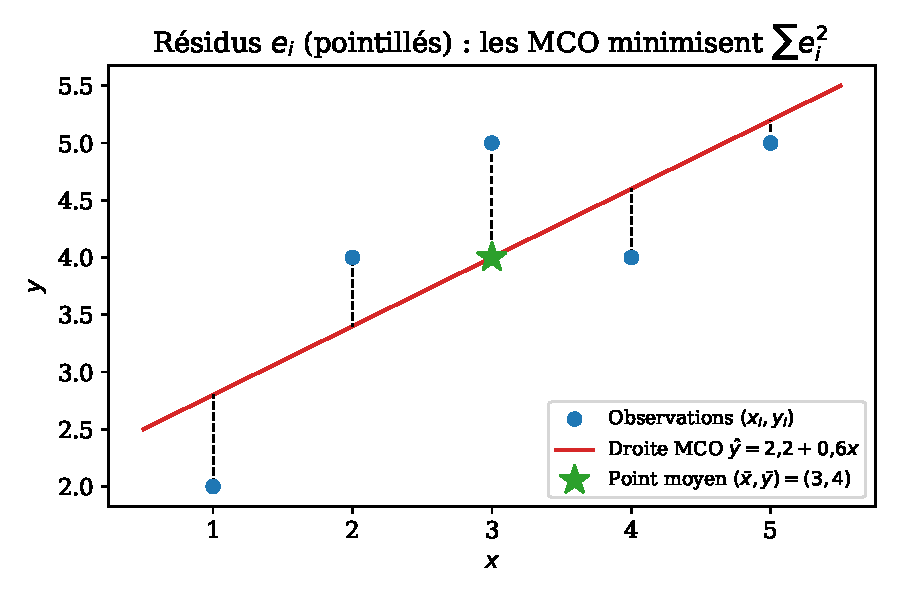
\includegraphics[width=0.72\textwidth]{figures/exemple_droite.pdf}
\caption{L'exemple numérique : la droite MCO passe par le point moyen et minimise la somme des carrés des segments verticaux.}
\end{figure}

\begin{histoire}
La méthode des moindres carrés a été publiée pour la première fois par \textbf{Adrien-Marie Legendre} en 1805, en annexe de ses \emph{Nouvelles méthodes pour la détermination des orbites des comètes} ; son exposé était purement algébrique. \textbf{Carl Friedrich Gauss} la publie en 1809 dans \emph{Theoria motus corporum coelestium} en affirmant l'utiliser depuis 1795 (il s'en serait servi en 1801 pour retrouver l'astéroïde Cérès), ce qui provoqua une célèbre querelle de priorité. L'apport de Gauss fut de donner à la méthode un fondement probabiliste : il montra qu'elle est optimale lorsque les erreurs suivent la loi qu'on appelle aujourd'hui « normale » ou « gaussienne ».
\end{histoire}

% ======================= 4. PROPRIETES NUMERIQUES =======================
\section{Propriétés numériques des MCO (Greene 3.2.3)}

\subsection{Numérique contre statistique}
\begin{itemize}
\item \textbf{Propriétés numériques} : vraies \emph{pour n'importe quel jeu de données}, par construction de l'algorithme. Elles ne demandent aucune hypothèse sur les erreurs. Exemple : « la somme des résidus est nulle ».
\item \textbf{Propriétés statistiques} : décrivent le comportement de $\vb$ \emph{en échantillons répétés} (espérance, variance, loi). Elles reposent sur des hypothèses sur la façon dont les données sont générées. Exemple : « $\vb$ est sans biais ».
\end{itemize}
\begin{intuition}
Une propriété numérique se vérifie sur votre fichier de données avec une calculatrice. Une propriété statistique ne peut pas se vérifier sur un seul échantillon : elle parle de ce qui se passerait si l'on recommençait l'expérience un grand nombre de fois (d'où l'intérêt de Monte Carlo, section~\ref{sec:mc}).
\end{intuition}

\subsection{Les équations normales [24] et l'orthogonalité [25]}
Les équations normales $\XtX\vb=\vX'\vy$ se réécrivent $\vX'(\vy-\vX\vb)=\mathbf 0$, c'est-à-dire
\[
\boxed{\vX'\ve=\mathbf 0}\qquad\Longleftrightarrow\qquad \sumi x_{ik}\,e_i=0\quad\text{pour chaque variable }k=1,\dots,K.
\]
(Les notes écrivent $\ve=\vX\vb-\vy$ en [24] ; la bonne définition est $\ve=\vy-\vX\vb$, mais le signe n'a pas d'importance puisque le résultat vaut zéro.)

\begin{intuition}
Chaque variable explicative est « non corrélée » (orthogonale) avec les résidus \emph{dans l'échantillon}. S'il restait une corrélation entre $x_k$ et $\ve$, on pourrait encore ajuster le coefficient de $x_k$ pour mieux prédire $y$ : on ne serait pas au minimum. Les résidus sont ce qui reste une fois que les $\vX$ ont « tout expliqué » de ce qu'elles pouvaient expliquer linéairement.
\end{intuition}

\begin{attention}
$\vX'\ve=\mathbf 0$ est une propriété \emph{numérique} toujours vraie. Elle ne dit \textbf{rien} sur l'hypothèse $\E[\veps\mid\vX]=\mathbf 0$ (erreurs non corrélées avec $\vX$ dans la population). On ne peut donc pas « tester l'exogénéité » en calculant la corrélation entre $\vX$ et les résidus : elle vaut zéro par construction !
\end{attention}

\subsection{Les conséquences quand le modèle contient une constante}
Si la première colonne de $\vX$ est $\vi=(1,\dots,1)'$, la première ligne de $\vX'\ve=\mathbf 0$ est $\vi'\ve=\sumi e_i=0$. On en déduit :
\begin{enumerate}
\item \textbf{Somme (et moyenne) des résidus nulle} : $\sum e_i=0$, $\bar e=0$.
\item \textbf{La régression passe par le point moyen} [27]--[29] : $\sum e_i=\sum(y_i-\vx_i'\vb)=0$, divisé par $n$ : $\bar y=\bar{\vx}'\vb$, où $\bar{\vx}$ est le vecteur des moyennes des variables. En bivarié : $\bar y=b_1+b_2\bar x$.
\item \textbf{Moyenne des prédictions = moyenne observée} [30]--[31] : puisque $\vy=\hat{\vy}+\ve$, on a $\sum y_i=\sum\hat y_i+\sum e_i=\sum\hat y_i$, donc $\bar{\hat y}=\bar y$.
\item (Complément) \textbf{Les prédictions sont orthogonales aux résidus} : $\hat{\vy}'\ve=\vb'\vX'\ve=0$.
\end{enumerate}

\begin{exemple}
Avec l'exemple : $\sum e_i=-0{,}8+0{,}6+1{,}0-0{,}6-0{,}2=0$ \checkmark ; \ $\sum x_ie_i=-0{,}8+1{,}2+3{,}0-2{,}4-1{,}0=0$ \checkmark ; \ $\bar{\hat y}=(2{,}8+3{,}4+4+4{,}6+5{,}2)/5=4=\bar y$ \checkmark.
\end{exemple}

\begin{attention}
Sans constante, ces propriétés 1--3 \textbf{ne tiennent plus} en général : les résidus ne somment pas à zéro et, comme on le verra, le $R^2$ usuel peut même devenir négatif. C'est une raison de toujours inclure une constante sauf justification théorique forte.
\end{attention}

% ======================= 5. PROJECTIONS =======================
\section{Les matrices de projection $\Pm$ et $\Mm$ (Greene 3.2.4)}

\subsection{Définitions}
En remplaçant $\vb$ par sa formule :
\[
\hat{\vy}=\vX\vb=\underbrace{\vX\XtXi\vX'}_{\Pm}\vy,\qquad
\ve=\vy-\hat{\vy}=\underbrace{(\I_n-\vX\XtXi\vX')}_{\Mm}\vy .
\]
$\Pm$ (« matrice chapeau », \emph{hat matrix}, car elle met un chapeau sur $\vy$) et $\Mm$ (« matrice créatrice de résidus », \emph{residual maker}) sont $n\times n$ et ne dépendent que de $\vX$.

\subsection{Démonstration des propriétés}
\begin{detail}
\textbf{Symétrie.} $\Pm'=(\vX\XtXi\vX')'=\vX\,[\XtXi]'\,\vX'=\vX\XtXi\vX'=\Pm$, car l'inverse d'une matrice symétrique est symétrique. Alors $\Mm'=\I'-\Pm'=\I-\Pm=\Mm$.

\textbf{Idempotence.} $\Pm\Pm=\vX\XtXi\underbrace{\vX'\vX\XtXi}_{=\I_K}\vX'=\vX\XtXi\vX'=\Pm$.
\\ $\Mm\Mm=(\I-\Pm)(\I-\Pm)=\I-2\Pm+\Pm\Pm=\I-2\Pm+\Pm=\I-\Pm=\Mm$.

\textbf{Action sur $\vX$.} $\Pm\vX=\vX\XtXi\XtX=\vX$ \ et \ $\Mm\vX=\vX-\Pm\vX=\mathbf 0$.

\textbf{Orthogonalité mutuelle.} $\Pm\Mm=\Pm-\Pm\Pm=\mathbf 0$.
\end{detail}

\begin{intuition}
\begin{itemize}[nosep]
\item \emph{Idempotente} : projeter deux fois = projeter une fois. Si on régresse $\hat{\vy}$ sur $\vX$, on retrouve $\hat{\vy}$ (il est déjà « dans » l'espace de $\vX$). Si on régresse les résidus $\ve$ sur $\vX$, on obtient des coefficients nuls et les mêmes résidus.
\item $\Pm\vX=\vX$ : régresser une variable explicative sur toutes les variables explicatives l'explique parfaitement.
\item $\Mm\vX=\mathbf 0$ : les résidus de cette régression sont nuls.
\end{itemize}
\end{intuition}

\subsection{Interprétation géométrique}
Voyons $\vy$ comme un point de $\mathbb R^n$. Les colonnes de $\vX$ engendrent un sous-espace de dimension $K$ (un « plan » si $K=2$). Les MCO cherchent le point $\vX\vb$ de ce plan le plus proche de $\vy$ au sens de la distance euclidienne ($S(\vb_0)=\|\vy-\vX\vb_0\|^2$). Le point le plus proche est le \textbf{pied de la perpendiculaire} : $\hat{\vy}=\Pm\vy$. Le résidu $\ve=\Mm\vy$ est le segment perpendiculaire au plan. C'est exactement le théorème de Pythagore qui donnera la décomposition de la variance.

\begin{figure}[h]
\centering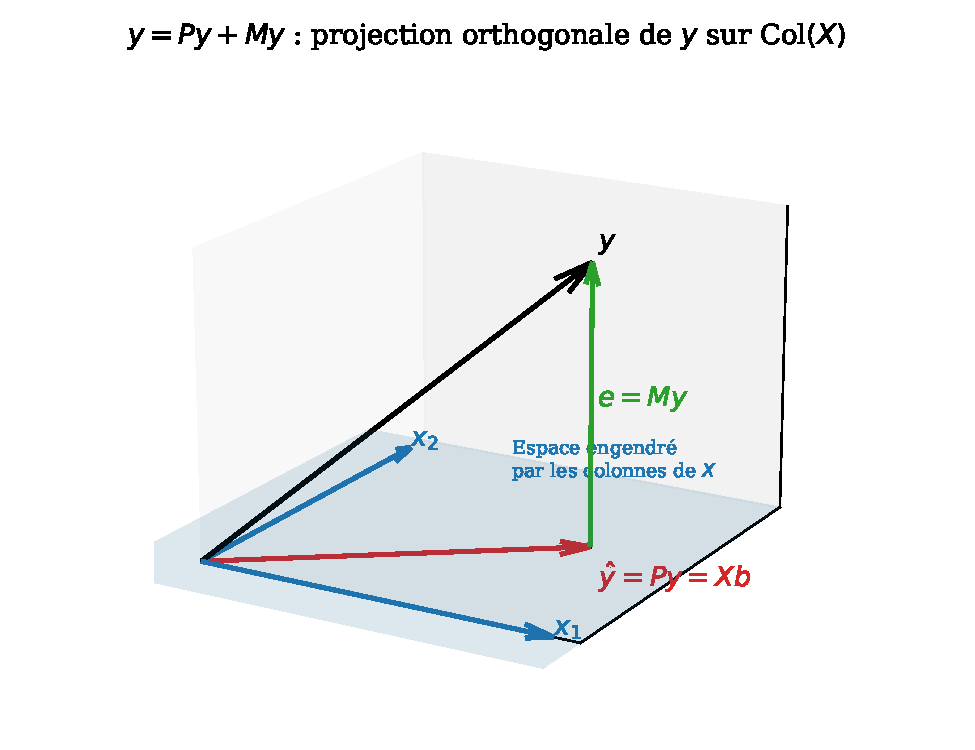
\includegraphics[width=0.66\textwidth]{figures/projection.pdf}
\caption{Géométrie des MCO avec $n=3$ et $K=2$ : $\hat{\vy}$ est l'ombre de $\vy$ sur le plan engendré par les colonnes de $\vX$ ; le résidu est perpendiculaire à ce plan.}
\end{figure}

\begin{resultat}
\begin{itemize}[nosep]
\item $\vy=\Pm\vy+\Mm\vy=\hat{\vy}+\ve$, avec $\hat{\vy}\perp\ve$.
\item Pythagore : $\vy'\vy=\hat{\vy}'\hat{\vy}+\ve'\ve$.
\item $\tr(\Pm)=K$ et $\tr(\Mm)=n-K$ (dimensions des deux sous-espaces ; voir §\ref{sec:sigma2}).
\item Les éléments diagonaux $p_{ii}$ de $\Pm$ s'appellent les \emph{leviers} (\emph{leverage}) : ils mesurent l'influence potentielle de l'observation $i$ sur sa propre prédiction.
\end{itemize}
\end{resultat}

% ======================= 6. FWL =======================
\section{Le théorème de Frisch-Waugh-Lovell (Greene 3.3)}

\subsection{Énoncé}
On partitionne $\vX=[\vX_1\ \vX_2]$ et $\vbeta=(\vbeta_1',\vbeta_2')'$ : $\vy=\vX_1\vbeta_1+\vX_2\vbeta_2+\veps$. On note $\Mm_1=\I-\vX_1(\vX_1'\vX_1)^{-1}\vX_1'$ la matrice qui crée les résidus d'une régression sur $\vX_1$.

\begin{theoreme}[FWL]
Le coefficient $\vb_2$ de la régression complète de $\vy$ sur $[\vX_1\ \vX_2]$ est identique au coefficient obtenu en :
\begin{enumerate}[nosep]
\item régressant $\vy$ sur $\vX_1$ et gardant les résidus $\tilde{\vy}=\Mm_1\vy$ ;
\item régressant chaque colonne de $\vX_2$ sur $\vX_1$ et gardant les résidus $\tilde{\vX}_2=\Mm_1\vX_2$ ;
\item régressant $\tilde{\vy}$ sur $\tilde{\vX}_2$ :
\ $\vb_2=(\tilde{\vX}_2'\tilde{\vX}_2)^{-1}\tilde{\vX}_2'\tilde{\vy}=(\vX_2'\Mm_1\vX_2)^{-1}\vX_2'\Mm_1\vy$.
\end{enumerate}
De plus, les résidus de l'étape 3 sont identiques aux résidus de la régression complète.
\end{theoreme}

\subsection{La démonstration complète (l'étape « après manipulation »)}
\begin{detail}
Les équations normales partitionnées [41] donnent
\begin{align*}
\vX_1'\vX_1\vb_1+\vX_1'\vX_2\vb_2&=\vX_1'\vy \qquad [42]\\
\vX_2'\vX_1\vb_1+\vX_2'\vX_2\vb_2&=\vX_2'\vy \qquad [43]
\end{align*}
De [42] : $\vb_1=(\vX_1'\vX_1)^{-1}\vX_1'(\vy-\vX_2\vb_2)$ \quad [45].

On remplace dans [43] :
\[
\vX_2'\vX_1(\vX_1'\vX_1)^{-1}\vX_1'(\vy-\vX_2\vb_2)+\vX_2'\vX_2\vb_2=\vX_2'\vy .
\]
Reconnaissons $\Pm_1=\vX_1(\vX_1'\vX_1)^{-1}\vX_1'$ :
\[
\vX_2'\Pm_1\vy-\vX_2'\Pm_1\vX_2\vb_2+\vX_2'\vX_2\vb_2=\vX_2'\vy
\ \Longrightarrow\
\vX_2'(\I-\Pm_1)\vX_2\,\vb_2=\vX_2'(\I-\Pm_1)\vy .
\]
Comme $\I-\Pm_1=\Mm_1$ : \ $\vX_2'\Mm_1\vX_2\,\vb_2=\vX_2'\Mm_1\vy$, d'où [46] :
\[
\vb_2=(\vX_2'\Mm_1\vX_2)^{-1}\vX_2'\Mm_1\vy .
\]
Enfin, comme $\Mm_1$ est symétrique et idempotente, $\vX_2'\Mm_1\vX_2=\vX_2'\Mm_1'\Mm_1\vX_2=(\Mm_1\vX_2)'(\Mm_1\vX_2)$ et $\vX_2'\Mm_1\vy=(\Mm_1\vX_2)'(\Mm_1\vy)$ : c'est bien la formule MCO de la régression de $\Mm_1\vy$ sur $\Mm_1\vX_2$.
\end{detail}

\begin{detail}[title={Remarque sur la seconde preuve du cours [47]--[49]}]
Le cours prémultiplie le modèle par $\Mm_1$ : $\Mm_1\vy=\Mm_1\vX_2\vbeta_2+\Mm_1\veps$ (car $\Mm_1\vX_1=\mathbf 0$). C'est un argument sur le \emph{modèle} (la population). La preuve rigoureuse, au niveau de l'\emph{estimateur}, fait la même chose sur la décomposition $\vy=\vX_1\vb_1+\vX_2\vb_2+\ve$ :
\[
\Mm_1\vy=\Mm_1\vX_2\vb_2+\Mm_1\ve=\Mm_1\vX_2\vb_2+\ve ,
\]
car $\ve$ est orthogonal à $\vX_1$ (donc $\Mm_1\ve=\ve$). En multipliant par $(\Mm_1\vX_2)'$ et en utilisant $\vX_2'\Mm_1\ve=\vX_2'\ve=\mathbf 0$, on retrouve [46]. Au passage, on voit que les résidus de l'étape 3 sont exactement $\ve$.
\end{detail}

\subsection{Pourquoi ce théorème est si important}
\begin{intuition}
$\Mm_1\vX_2$ est la partie de $\vX_2$ \emph{que $\vX_1$ ne peut pas expliquer}. Le coefficient $\vb_2$ n'utilise donc que la variation de $\vX_2$ « nettoyée » de $\vX_1$ : c'est la traduction mathématique précise de l'expression \textbf{« toutes choses égales par ailleurs »} (\emph{ceteris paribus}). Dans l'équation de salaire, le coefficient de la scolarité mesure l'association entre salaire et la partie de la scolarité non prédite par l'expérience.
\end{intuition}

Applications classiques :
\begin{itemize}
\item \textbf{Tendance temporelle} (le cas étudié par Frisch et Waugh en 1933) : régresser $y$ sur $x$ et une tendance $t$ donne le même coefficient de $x$ que régresser $y$ « détendancié » sur $x$ « détendancié ».
\item \textbf{Constante} : si $\vX_1=\vi$, $\Mm_1=\Mm^0$ centre les variables. Donc la pente d'une régression avec constante = pente de la régression \emph{sans constante} des variables centrées. C'est pourquoi la formule bivariée [16] fait intervenir $x_i-\bar x$ et $y_i-\bar y$.
\item \textbf{Effets fixes} (données de panel) : inclure une indicatrice par individu revient à retirer à chaque variable sa moyenne individuelle (estimateur « within »).
\item \textbf{Graphiques de régression partielle} (\emph{added-variable plots}) : on représente $\Mm_1\vy$ contre $\Mm_1\vx_2$ ; la pente de ce nuage est exactement $b_2$.
\item \textbf{Biais de variable omise} : si on omet $\vX_2$, on estime $\vb_1^{\text{court}}=(\vX_1'\vX_1)^{-1}\vX_1'\vy$. Par [45], $\vb_1^{\text{court}}=\vb_1+(\vX_1'\vX_1)^{-1}\vX_1'\vX_2\,\vb_2$ : l'écart est nul seulement si $\vX_2$ n'a pas d'effet ($\vb_2=\mathbf 0$) ou si $\vX_1\perp\vX_2$.
\end{itemize}

\begin{exemple}[title={Vérification numérique (simulation, $n=200$)}]
Modèle $y=1+2x_1-x_2+\epsilon$ avec $x_2=0{,}7x_1+u$ (variables corrélées). La régression complète donne $b_2=-1{,}17573366$ ; la procédure FWL en trois étapes donne $b_2=-1{,}17573366$. Identiques à la dernière décimale, comme le théorème l'affirme.
\end{exemple}

\begin{attention}
Les \emph{coefficients} sont identiques, mais l'écart-type affiché par le logiciel à l'étape 3 est légèrement faux : il divise la somme des carrés des résidus par $n-K_2$ au lieu de $n-K$ (il « ignore » que $K_1$ paramètres ont été estimés à l'étape 1). Il faut corriger par le facteur $\sqrt{(n-K_2)/(n-K)}$.
\end{attention}

\begin{histoire}
Le résultat remonte en fait à \textbf{George Udny Yule} (1907), qui analysait déjà les régressions partielles. \textbf{Ragnar Frisch} (premier prix Nobel d'économie, 1969) et \textbf{Frederick Waugh} l'établissent en 1933 dans « Partial Time Regressions as Compared with Individual Trends » (\emph{Econometrica}), avec une preuve par déterminants et règle de Cramer, pour montrer qu'on peut soit inclure une tendance, soit détendancier les séries. \textbf{Michael Lovell} (1963, \emph{JASA}) généralise le résultat et en donne la preuve matricielle simple par projections, d'où le nom « FWL » (certains auteurs disent désormais « YFWL »).
\end{histoire}

% ======================= 7. R2 =======================
\section{Le coefficient de détermination $R^2$ (Greene 3.5)}

\subsection{La matrice $\Mm^0$ qui centre}
$\Mm^0=\I_n-\vi(\vi'\vi)^{-1}\vi'=\I_n-\frac1n\vi\vi'$ est la matrice $\Mm$ de la régression sur une constante seule. Or la régression de $\vy$ sur une constante donne $b=\bar y$ (la moyenne), donc les résidus sont $y_i-\bar y$ :
\[
\Mm^0\vy=\big(y_1-\bar y,\dots,y_n-\bar y\big)' ,\qquad \Pm^0\vy=(\bar y,\dots,\bar y)'.
\]
C'est ce que l'exemple $n=3$ du cours [53]--[57] vérifie à la main. Comme toute matrice $\Mm$, $\Mm^0$ est symétrique et idempotente, d'où
\[
\vy'\Mm^0\vy=(\Mm^0\vy)'(\Mm^0\vy)=\sumi(y_i-\bar y)^2 .
\]

\subsection{La décomposition SCT = SCR + SCE [58]--[66]}
\begin{detail}
Partons de $\vy=\vX\vb+\ve$ et multiplions par $\Mm^0$ : $\Mm^0\vy=\Mm^0\vX\vb+\Mm^0\ve$.
Avec une constante, $\bar e=0$, donc $\Mm^0\ve=\ve-\bar e\vi=\ve$. Ainsi $\Mm^0\vy=\Mm^0\vX\vb+\ve$. On calcule le carré de la norme :
\[
\vy'\Mm^0\vy=\vb'\vX'\Mm^0\vX\vb+2\,\vb'\vX'\Mm^0\ve+\ve'\ve .
\]
Le terme croisé est nul : $\vX'\Mm^0\ve=\vX'\ve=\mathbf 0$. Donc
\[
\underbrace{\sumi(y_i-\bar y)^2}_{\text{SCT}}=\underbrace{\sumi(\hat y_i-\bar y)^2}_{\text{SCR}}+\underbrace{\sumi e_i^2}_{\text{SCE}} .
\]
(Pour SCR : $\Mm^0\vX\vb=\Mm^0\hat{\vy}$ est le vecteur des $\hat y_i-\bar{\hat y}=\hat y_i-\bar y$.)
\end{detail}

\begin{intuition}
C'est Pythagore dans l'espace des variables centrées : la variation totale de $y$ autour de sa moyenne se décompose en une partie « expliquée » par la régression et une partie « inexpliquée » (résiduelle), sans terme croisé car $\hat{\vy}\perp\ve$.
\end{intuition}

\begin{attention}[title={Attention aux sigles !}]
Les notes utilisent les sigles français : SCR = somme des carrés de la \emph{régression} (expliquée), SCE = somme des carrés des \emph{erreurs} (résidus). Or en anglais, selon les manuels, \emph{SSR} désigne tantôt « \emph{sum of squared residuals} » (= notre SCE !) tantôt « \emph{regression sum of squares} », et \emph{SSE} tantôt « \emph{explained} » tantôt « \emph{error} ». Les notes elles-mêmes passent de SCE à « SSE » en section 2.4.1. Toujours vérifier la définition utilisée plutôt que le sigle.
\end{attention}

\subsection{Définition et interprétation du $R^2$}
\[
R^2=\frac{\text{SCR}}{\text{SCT}}=1-\frac{\text{SCE}}{\text{SCT}}=1-\frac{\ve'\ve}{\vy'\Mm^0\vy}\in[0,1]\quad(\text{avec constante}).
\]
\begin{itemize}
\item Proportion de la variance de $y$ expliquée (linéairement) par les $x$.
\item Propriété utile : $R^2=\big[\widehat{\text{corr}}(y,\hat y)\big]^2$ ; en bivarié, $R^2=\big[\widehat{\text{corr}}(x,y)\big]^2$.
\item Un $R^2$ faible ne veut pas dire que le modèle est « faux » ni que les coefficients sont mal estimés (en microéconomie appliquée, $R^2\approx0{,}1$ est courant). Un $R^2$ élevé ne veut pas dire qu'on a un effet causal (deux séries avec tendance ont souvent un $R^2$ énorme : régression fallacieuse).
\end{itemize}

\begin{exemple}
SCT $=\sum(y_i-4)^2=4+0+1+0+1=6$ ; SCE $=0{,}64+0{,}36+1+0{,}36+0{,}04=2{,}4$ ; SCR $=\sum(\hat y_i-4)^2=1{,}44+0{,}36+0+0{,}36+1{,}44=3{,}6$. On vérifie $6=3{,}6+2{,}4$ \checkmark, et $R^2=3{,}6/6=0{,}6$.
\end{exemple}

\begin{attention}
Sans constante, $\Mm^0\ve\ne\ve$ en général, la décomposition échoue et $1-\text{SCE}/\text{SCT}$ peut être \textbf{négatif}. Les logiciels rapportent alors un « $R^2$ non centré » ($1-\ve'\ve/\vy'\vy$), qui n'est pas comparable au $R^2$ usuel.
\end{attention}

\subsection{Pourquoi le $R^2$ augmente quand on ajoute une variable [68]--(fin 2.4.1)}
Le résultat : si l'on ajoute une variable $\vx_2$ à $\vX_1$,
\[
\boxed{\ \text{SCE}_2=\text{SCE}_1-\tilde b_2^{\,2}\,\vx_2'\Mm_1\vx_2\ \le\ \text{SCE}_1\ }
\]

\begin{detail}[title={La démonstration en version courte (via FWL)}]
Par FWL, les résidus du grand modèle s'obtiennent en régressant $\ve_1=\Mm_1\vy$ sur $\tilde{\vx}_2=\Mm_1\vx_2$ : \ $\ve_2=\ve_1-\tilde{\vx}_2\tilde b_2$ avec $\tilde b_2=\tilde{\vx}_2'\ve_1/\tilde{\vx}_2'\tilde{\vx}_2$. Donc
\[
\ve_2'\ve_2=\ve_1'\ve_1-2\tilde b_2\,\tilde{\vx}_2'\ve_1+\tilde b_2^{\,2}\,\tilde{\vx}_2'\tilde{\vx}_2 .
\]
Or $\tilde{\vx}_2'\ve_1=\tilde b_2\,\tilde{\vx}_2'\tilde{\vx}_2$ (définition de $\tilde b_2$). D'où
$\ve_2'\ve_2=\ve_1'\ve_1-\tilde b_2^{\,2}\,\tilde{\vx}_2'\tilde{\vx}_2=\ve_1'\ve_1-\tilde b_2^{\,2}\,\vx_2'\Mm_1\vx_2$.
Comme $\vx_2'\Mm_1\vx_2=\|\Mm_1\vx_2\|^2\ge0$ et $\tilde b_2^{\,2}\ge0$, la SCE ne peut que baisser (ou rester égale si $\tilde b_2=0$).

La démonstration longue du cours [75]--[76] fait exactement ce calcul, en développant le carré et en montrant que le terme du milieu $-2\tilde b_2\vx_2'\Mm_1\ve_1$ vaut $-2\tilde b_2^{\,2}\vx_2'\Mm_1\vx_2$.
\end{detail}

\begin{intuition}
Argument sans calcul : le grand modèle peut toujours reproduire le petit en posant $\tilde b_2=0$. Minimiser sur un ensemble plus grand ne peut donner qu'un minimum plus petit ou égal. Ajouter n'importe quelle variable, même générée au hasard, fait donc baisser SCE et monter $R^2$. Avec $K=n$ variables (plein rang), l'ajustement est parfait : $R^2=1$.
\end{intuition}

\begin{figure}[h]
\centering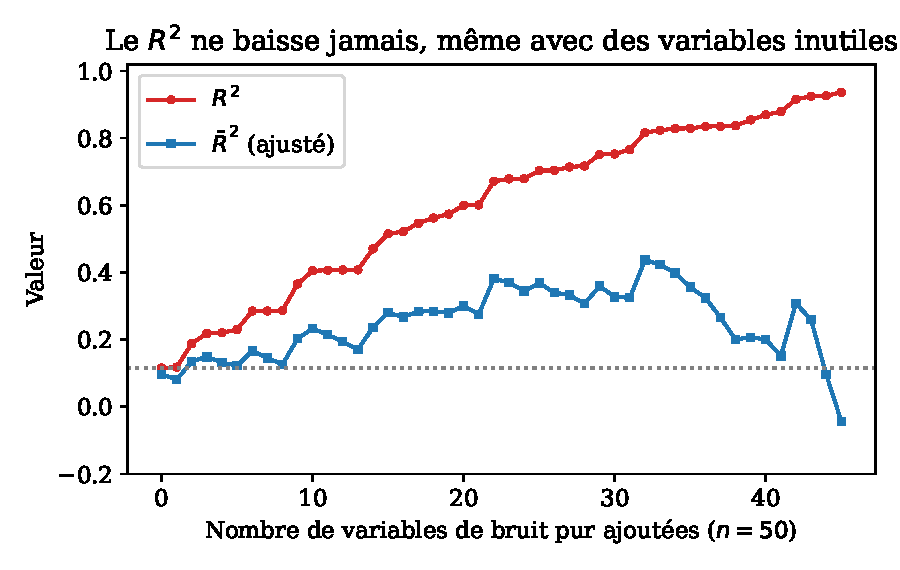
\includegraphics[width=0.72\textwidth]{figures/r2_bruit.pdf}
\caption{Simulation ($n=50$) : le vrai modèle n'a qu'une variable. On ajoute une à une 45 variables de pur bruit. Le $R^2$ passe de 0,12 à 0,94 alors qu'aucune de ces variables n'a de lien avec $y$ ; le $R^2$ ajusté, lui, stagne puis devient négatif.}
\end{figure}

\subsection{Complément : le $R^2$ ajusté et les critères d'information}
Pour comparer des modèles ayant des nombres de variables différents, on pénalise le nombre de paramètres (Theil, 1961) :
\[
\bar R^2=1-\frac{\text{SCE}/(n-K)}{\text{SCT}/(n-1)}=1-\frac{n-1}{n-K}(1-R^2).
\]
Il n'augmente lorsqu'on ajoute une variable que si la baisse de SCE « paie » la perte d'un degré de liberté (on peut montrer : si et seulement si la statistique $t$ de la nouvelle variable est supérieure à 1 en valeur absolue). Des critères plus exigeants existent : AIC $=\ln(\text{SCE}/n)+2K/n$ et BIC (ou critère de Schwarz) $=\ln(\text{SCE}/n)+K\ln(n)/n$ (Greene, ch.~5).

% ======================= 8. PROPRIETES STATISTIQUES =======================
\section{Propriétés statistiques des MCO (Greene 4.1--4.3)}

\subsection{Les hypothèses du modèle classique, une par une}
\begin{center}
\renewcommand{\arraystretch}{1.3}
\begin{tabular}{@{}p{3.6cm}p{5.4cm}p{5.6cm}@{}}
\toprule
Hypothèse & Signification & Exemple de violation \\
\midrule
H1 Linéarité & $\vy=\vX\vbeta+\veps$ : linéaire \emph{dans les paramètres} ($x^2$, $\ln x$ sont permis) & $y=\beta_1 x^{\beta_2}+\epsilon$ (non linéaire en $\beta_2$) \\
H2 Plein rang & aucune colinéarité parfaite ; $\XtX$ inversible & piège des indicatrices ; $n<K$ \\
H3 Exogénéité $\E[\veps\mid\vX]=\mathbf 0$ & les $\vX$ ne contiennent aucune information sur les erreurs & variable omise corrélée (habileté et scolarité), simultanéité, erreur de mesure sur $x$ \\
H4 $\E[\veps\veps'\mid\vX]=\sigma^2\I_n$ & homoscédasticité (même variance) et absence d'autocorrélation & variance du revenu qui croît avec le revenu ; chocs persistants en séries temporelles \\
H5 Normalité & $\veps\mid\vX\sim N(\mathbf 0,\sigma^2\I_n)$ & erreurs asymétriques ou à queues épaisses \\
\bottomrule
\end{tabular}
\end{center}

Lecture de H4 : l'élément $(i,j)$ de $\veps\veps'$ est $\epsilon_i\epsilon_j$. Donc $\E[\epsilon_i^2\mid\vX]=\sigma^2$ (diagonale : même variance pour tous) et $\E[\epsilon_i\epsilon_j\mid\vX]=0$ pour $i\ne j$ (hors diagonale : pas de corrélation entre observations).

\begin{resultat}
\begin{itemize}[nosep]
\item Absence de biais : H1, H2, H3.
\item Formule de variance $\sigma^2\XtXi$ et Gauss-Markov : H1--H4.
\item Loi exacte (normale) de $\vb$, tests $t$ et $F$ exacts en petit échantillon : H1--H5.
\end{itemize}
\end{resultat}

\subsection{Absence de biais [79]--[80]}
\begin{detail}
Étape 1 — écrire l'estimateur en fonction de l'erreur (substituer le vrai modèle) :
\[
\vb=\XtXi\vX'(\vX\vbeta+\veps)=\underbrace{\XtXi\XtX}_{\I_K}\vbeta+\XtXi\vX'\veps=\vbeta+\XtXi\vX'\veps .
\]
Cette « décomposition de l'erreur d'échantillonnage » $\vb-\vbeta=\XtXi\vX'\veps$ est la clé de \emph{toutes} les preuves qui suivent.

Étape 2 — prendre l'espérance conditionnelle à $\vX$ : conditionnellement à $\vX$, la matrice $\XtXi\vX'$ est une constante et sort de l'espérance :
\[
\E[\vb\mid\vX]=\vbeta+\XtXi\vX'\E[\veps\mid\vX]=\vbeta+\mathbf 0=\vbeta .
\]
Étape 3 (complément) — loi des espérances itérées : $\E[\vb]=\E\big[\E[\vb\mid\vX]\big]=\E[\vbeta]=\vbeta$. L'estimateur est donc sans biais aussi inconditionnellement.
\end{detail}

\begin{intuition}
« Sans biais » ne veut pas dire que $\vb=\vbeta$ dans votre échantillon ! Cela veut dire que si l'on répétait l'expérience une infinité de fois, la moyenne des $\vb$ obtenus serait $\vbeta$ : l'estimateur ne se trompe pas \emph{systématiquement} dans une direction. L'étude de Monte Carlo (section~\ref{sec:mc}) le visualise.
\end{intuition}

\begin{attention}
Si H3 échoue (par exemple une variable omise corrélée avec $\vX$), $\E[\veps\mid\vX]\ne\mathbf 0$ et $\vb$ est biaisé — et ce biais ne disparaît pas quand $n$ augmente. C'est le problème central de l'économétrie appliquée (d'où les variables instrumentales, plus tard dans le cours).
\end{attention}

\subsection{Variance [81]--[82]}
\begin{detail}
Par définition, $\Var(\vb\mid\vX)=\E[(\vb-\vbeta)(\vb-\vbeta)'\mid\vX]$, une matrice $K\times K$ : la diagonale contient les variances des $b_k$, hors diagonale les covariances.
\begin{align*}
(\vb-\vbeta)(\vb-\vbeta)'&=\big(\XtXi\vX'\veps\big)\big(\XtXi\vX'\veps\big)'\\
&=\XtXi\vX'\veps\,\veps'\vX\,\big[\XtXi\big]' &&(\A\mathbf{B})'=\mathbf{B}'\A'\\
&=\XtXi\vX'\veps\veps'\vX\XtXi &&\XtXi\text{ symétrique}.
\end{align*}
Espérance conditionnelle (tout sauf $\veps\veps'$ est constant sachant $\vX$) puis H4 :
\[
\Var(\vb\mid\vX)=\XtXi\vX'\underbrace{\E[\veps\veps'\mid\vX]}_{\sigma^2\I_n}\vX\XtXi=\sigma^2\XtXi\XtX\XtXi=\sigma^2\XtXi .
\]
\end{detail}

\begin{exemple}[title={Cas bivarié : ce qui rend un estimateur précis}]
En bivarié, l'élément de $\sigma^2\XtXi$ correspondant à la pente est
\[
\Var(b_2\mid\vX)=\frac{\sigma^2}{\sumi(x_i-\bar x)^2}=\frac{\sigma^2}{n\,\widehat{\Var}(x)} .
\]
La pente est estimée plus précisément quand : (i) les erreurs sont peu dispersées ($\sigma^2$ petit) ; (ii) on a beaucoup d'observations ($n$ grand) ; (iii) $x$ varie beaucoup dans l'échantillon. Avec plusieurs variables, on montre (via FWL) que $\Var(b_k\mid\vX)=\sigma^2/\big[(1-R_k^2)\sum(x_{ik}-\bar x_k)^2\big]$, où $R_k^2$ est le $R^2$ de la régression de $x_k$ sur les autres variables : la \textbf{multicolinéarité} (non parfaite) gonfle la variance. Le facteur $1/(1-R_k^2)$ s'appelle le VIF (\emph{variance inflation factor}).
\end{exemple}

% ======================= 9. GAUSS-MARKOV =======================
\section{Le théorème de Gauss-Markov (Greene 4.3.5)}

\begin{theoreme}
Sous H1--H4, l'estimateur MCO $\vb$ est le \textbf{meilleur estimateur linéaire sans biais} (BLUE : \emph{Best Linear Unbiased Estimator}) : pour tout autre estimateur linéaire sans biais $\vb^*$, la matrice $\Var(\vb^*\mid\vX)-\Var(\vb\mid\vX)$ est semi-définie positive.
\end{theoreme}

\subsection{Décortiquer l'énoncé}
\begin{itemize}
\item \textbf{Linéaire} : $\vb^*=\C\vy$, avec $\C$ ($K\times n$) qui peut dépendre de $\vX$ mais pas de $\vy$. Les MCO en font partie avec $\C=\XtXi\vX'$. Autres exemples : n'utiliser que la moitié des observations ; en bivarié, la pente entre le premier et le dernier point $(y_n-y_1)/(x_n-x_1)$ ; les moindres carrés pondérés.
\item \textbf{Sans biais} : $\E[\C\vy\mid\vX]=\C\vX\vbeta+\C\,\E[\veps\mid\vX]=\C\vX\vbeta$. Pour que cela vaille $\vbeta$ \emph{quel que soit} $\vbeta$, il faut $\C\vX=\I_K$.
\item \textbf{Meilleur} : de plus petite variance, au sens matriciel.
\end{itemize}

\begin{attention}
Coquille dans les notes : il est écrit $\C\vX=\I_n$. Or $\C$ est $K\times n$ et $\vX$ est $n\times K$, donc $\C\vX$ est $K\times K$ : la condition correcte est $\C\vX=\I_K$ (idem pour [87]--[90]).
\end{attention}

\subsection{La preuve, étape par étape}
\begin{detail}
\textbf{1. Variance de $\vb^*$.} Avec $\C\vX=\I_K$ : $\vb^*=\C(\vX\vbeta+\veps)=\vbeta+\C\veps$, donc
$\Var(\vb^*\mid\vX)=\E[\C\veps\veps'\C'\mid\vX]=\C(\sigma^2\I)\C'=\sigma^2\C\C'$.

\textbf{2. Écrire $\C$ comme « MCO + écart ».} $\D=\C-\XtXi\vX'$, soit $\C=\D+\XtXi\vX'$.

\textbf{3. Contrainte sur $\D$.} $\C\vX=\D\vX+\XtXi\XtX=\D\vX+\I_K=\I_K$ \ $\Rightarrow$ \ $\D\vX=\mathbf 0$ (et en transposant, $\vX'\D'=\mathbf 0$).

\textbf{4. Développer $\C\C'$.}
\[
\begin{aligned}
\C\C'&=\big(\D+\XtXi\vX'\big)\big(\D'+\vX\XtXi\big)\\
&=\D\D'+\underbrace{\D\vX}_{\mathbf 0}\XtXi+\XtXi\underbrace{\vX'\D'}_{\mathbf 0}+\XtXi\XtX\XtXi .
\end{aligned}
\]
Donc $\C\C'=\D\D'+\XtXi$ et
\[
\Var(\vb^*\mid\vX)=\sigma^2\XtXi+\sigma^2\D\D'=\Var(\vb\mid\vX)+\sigma^2\D\D' .
\]
\textbf{5. Conclusion.} $\D\D'$ est semi-définie positive (§1.5), donc la variance de $\vb^*$ dépasse celle de $\vb$ d'une matrice « positive ». Égalité seulement si $\D=\mathbf 0$, c'est-à-dire $\vb^*=\vb$.
\end{detail}

\begin{intuition}
« $\Var(\vb^*)-\Var(\vb)$ semi-définie positive » implique en particulier que \textbf{chaque} coefficient est estimé avec une variance plus faible par MCO ($\Var(b_k)\le\Var(b_k^*)$, en prenant $\mathbf c=$ vecteur unitaire $k$), et plus généralement toute combinaison linéaire $\mathbf c'\vbeta$ (une prévision, un effet marginal) est estimée au mieux par $\mathbf c'\vb$.
\end{intuition}

\subsection{Ce que le théorème ne dit pas}
\begin{itemize}
\item Il ne compare les MCO qu'aux estimateurs \emph{linéaires} et \emph{sans biais}. Un estimateur biaisé (par exemple la régression « ridge » ou LASSO en apprentissage automatique) peut avoir une erreur quadratique moyenne plus faible.
\item Il ne requiert \emph{pas} la normalité (H5). Sous normalité, on a un résultat plus fort : les MCO sont les meilleurs parmi \emph{tous} les estimateurs sans biais, linéaires ou non (borne de Cramér-Rao).
\item Si H4 échoue (hétéroscédasticité, autocorrélation), les MCO restent sans biais mais ne sont plus BLUE : c'est l'estimateur des moindres carrés généralisés (MCG) qui l'est (théorème d'Aitken, 1935). De plus, la formule $\sigma^2\XtXi$ devient fausse (d'où les écarts-types « robustes » de White).
\end{itemize}

\begin{histoire}
Gauss a démontré ce résultat en 1821--1823 (\emph{Theoria combinationis observationum}), sans supposer la normalité. \textbf{Andreï Markov} le redémontre dans son manuel de probabilités de 1900. \textbf{Alexander Aitken} (1935) l'étend aux erreurs de matrice de variance quelconque (MCG). Bruce Hansen a récemment (\emph{Econometrica}, 2022) proposé une « version moderne » du théorème qui retire la restriction aux estimateurs linéaires, ce qui a suscité un débat dans la littérature.
\end{histoire}

% ======================= 10. SIGMA2 =======================
\section{L'estimation de $\sigma^2$ (Greene 4.3.4)}\label{sec:sigma2}

\subsection{Le problème}
$\Var(\vb\mid\vX)=\sigma^2\XtXi$ contient $\sigma^2$, inconnu. L'idée naturelle serait $\frac1n\sum e_i^2$, l'analogue empirique de $\frac1n\sum\epsilon_i^2$. Mais les résidus sont systématiquement « trop petits » : les MCO choisissent $\vb$ \emph{pour} minimiser $\sum e_i^2$, donc $\sum e_i^2\le\sum\epsilon_i^2$ (le vrai $\vbeta$ est un candidat parmi d'autres !).

\subsection{Calcul de $\E[\ve'\ve\mid\vX]$ [94]--[106]}
\begin{detail}
\textbf{1. Les résidus en fonction des erreurs.} $\ve=\Mm\vy=\Mm(\vX\vbeta+\veps)=\Mm\veps$ car $\Mm\vX=\mathbf 0$. Donc $\ve'\ve=\veps'\Mm'\Mm\veps=\veps'\Mm\veps$.

\textbf{2. L'astuce de la trace.} $\veps'\Mm\veps$ est un scalaire, donc égal à sa trace, et par permutation circulaire :
$\veps'\Mm\veps=\tr(\veps'\Mm\veps)=\tr(\Mm\veps\veps')$.
L'intérêt : on a regroupé les $\veps$ en $\veps\veps'$, dont on connaît l'espérance.

\textbf{3. Espérance.} La trace est une somme, donc linéaire, et commute avec l'espérance :
$\E[\tr(\Mm\veps\veps')\mid\vX]=\tr\big(\Mm\,\E[\veps\veps'\mid\vX]\big)=\tr(\Mm\,\sigma^2\I_n)=\sigma^2\tr(\Mm)$.

\textbf{4. Trace de $\Mm$.}
$\tr(\Mm)=\tr(\I_n)-\tr\big(\vX\XtXi\vX'\big)=n-\tr\big(\XtXi\vX'\vX\big)=n-\tr(\I_K)=n-K$.
(On a permuté $\vX$ de la première à la dernière position : la matrice passe de $n\times n$ à $K\times K$.)

\textbf{Conclusion.} $\E[\ve'\ve\mid\vX]=(n-K)\sigma^2$.
\end{detail}

\begin{resultat}
\[
s^2=\frac{\ve'\ve}{n-K}\quad\text{est sans biais pour }\sigma^2,
\]
\[
\widehat{\Var}(\vb\mid\vX)=s^2\XtXi,\qquad
\text{e.t.}(b_k)=\sqrt{s^2\,[\XtXi]_{kk}} .
\]
$s=\sqrt{s^2}$ s'appelle l'\emph{erreur-type de la régression} (« Root MSE » dans Stata, « Residual standard error » dans R).
\end{resultat}

\begin{intuition}[title={Intuition : les degrés de liberté}]
Les $n$ résidus ne sont pas libres : ils doivent satisfaire les $K$ équations $\vX'\ve=\mathbf 0$. Il ne reste donc que $n-K$ « degrés de liberté ». Géométriquement, $\ve=\Mm\veps$ vit dans un sous-espace de dimension $n-K$ (celui orthogonal à $\vX$) : il ne capte que $n-K$ des $n$ « directions » de variation de $\veps$, chacune d'espérance $\sigma^2$. C'est le même phénomène que le $n-1$ de la variance empirique $\frac1{n-1}\sum(x_i-\bar x)^2$, qui est le cas particulier $K=1$ (régression sur une constante).
\end{intuition}

\begin{exemple}
SCE $=2{,}4$, $n-K=5-2=3$, donc $s^2=0{,}8$. \ $\widehat{\Var}(\vb)=0{,}8\times\frac1{50}\begin{pmatrix}55&-15\\-15&5\end{pmatrix}=\begin{pmatrix}0{,}88&-0{,}24\\-0{,}24&0{,}08\end{pmatrix}$.
\\Écarts-types : e.t.$(b_1)=\sqrt{0{,}88}\approx0{,}938$, e.t.$(b_2)=\sqrt{0{,}08}\approx0{,}283$. La statistique $t$ de la pente est $0{,}6/0{,}283\approx2{,}12$. (Vérifiable avec \texttt{reg y x} dans Stata ou \texttt{lm(y\textasciitilde x)} dans R.)
\end{exemple}

\begin{attention}
$s^2$ est sans biais pour $\sigma^2$, mais $s$ est (légèrement) \emph{biaisé} pour $\sigma$ : la racine est concave, donc $\E[s]\le\sqrt{\E[s^2]}=\sigma$ (inégalité de Jensen). L'absence de biais ne se conserve pas par transformation non linéaire. De même, les écarts-types estimés ne sont pas exactement sans biais, mais le biais est négligeable (voir Monte Carlo).
\end{attention}

% ======================= 11. MONTE CARLO =======================
\section{Les études de Monte Carlo (Greene 15.5)}\label{sec:mc}

\subsection{Principe}
Une propriété statistique (sans biais, variance, loi) décrit ce qui se passe \emph{en échantillons répétés}. Dans la réalité, on n'observe qu'un seul échantillon et on ne connaît pas $\vbeta$. En simulation, on \textbf{fabrique} le monde : on choisit $\vbeta$ et $\sigma^2$, on génère des milliers d'échantillons, on estime sur chacun, et on regarde la distribution des estimations. C'est un « laboratoire » où la vérité est connue.

Utilité : vérifier un résultat théorique (comme ici), étudier des situations où la théorie est trop difficile (petits échantillons, estimateurs non linéaires, violations d'hypothèses), et introduction au \emph{bootstrap}.

\begin{histoire}
La méthode a été formalisée à Los Alamos vers 1946--1949 par \textbf{Stanislaw Ulam} et \textbf{John von Neumann} (avec Nicholas Metropolis, qui trouva le nom en référence au casino de Monaco), pour simuler la diffusion des neutrons sur les premiers ordinateurs (ENIAC). Ulam en eut l'idée en se demandant quelle était la probabilité de réussir une patience aux cartes.
\end{histoire}

\subsection{Générer des nombres (pseudo-)aléatoires [110]}
Un ordinateur est déterministe ; il produit des suites qui \emph{ressemblent} à du hasard. Le générateur congruentiel linéaire (GCL) :
\[
x_t=(\alpha+\lambda x_{t-1})\bmod m,\qquad u_t=x_t/m\in[0,1).
\]
$a\bmod b$ est le reste de la division entière de $a$ par $b$ (par ex.\ $17\bmod 5=2$).

\begin{exemple}[title={Un GCL « jouet » calculé à la main}]
$\alpha=3$, $\lambda=5$, $m=16$, graine $x_0=7$ :
$x_1=(3+35)\bmod16=38\bmod16=6$ ; \ $x_2=(3+30)\bmod16=1$ ; \ $x_3=(3+5)\bmod16=8$ ; \ $x_4=43\bmod16=11$ ; \dots
\\ La suite complète : 6, 1, 8, 11, 10, 5, 12, 15, 14, 9, 0, 3, 2, 13, 4, 7, \textbf{6, 1, 8, \dots}
\\ Après 16 termes, on retombe sur 7 puis la suite \textbf{se répète} : la \emph{période} est au plus $m$. C'est pourquoi on prend $m$ très grand ($2^{31}-1$, $2^{63}-1$\dots). Et la même graine redonne toujours la même suite : c'est ce qui rend les simulations \textbf{reproductibles}.
\end{exemple}

\begin{attention}
Les GCL ont des défauts : les $k$-uplets successifs $(u_t,u_{t+1},u_{t+2})$ se rangent sur un petit nombre d'hyperplans (théorème de Marsaglia, 1968). Le célèbre générateur RANDU d'IBM (années 1960) plaçait tous les triplets sur seulement 15 plans, ce qui a jeté le doute sur de nombreux résultats de simulation de l'époque. Les logiciels modernes utilisent de meilleurs générateurs : Stata (depuis la v.~14) et R utilisent par défaut le \emph{Mersenne Twister} (période $2^{19937}-1$). Le principe (graine, suite déterministe) reste le même.
\end{attention}

\subsection{Obtenir n'importe quelle loi : la transformation inverse}
Si $U\sim U[0,1]$ et $F$ est une fonction de répartition (continue, strictement croissante), alors $X=F^{-1}(U)$ suit la loi $F$.

\begin{detail}[title={Pourquoi ça marche (une ligne)}]
$P(X\le x)=P(F^{-1}(U)\le x)=P(U\le F(x))=F(x)$, car pour une uniforme $P(U\le a)=a$.
\end{detail}
\begin{exemple}
Loi exponentielle de paramètre $\lambda$ : $F(x)=1-e^{-\lambda x}$. On résout $u=1-e^{-\lambda x}$ : $x=-\ln(1-u)/\lambda$. Pour la loi normale, $F^{-1}=\Phi^{-1}$ n'a pas de formule explicite ; on l'approxime numériquement, ou on utilise la méthode de Box-Muller : $Z=\sqrt{-2\ln U_1}\cos(2\pi U_2)$ est $N(0,1)$.
\end{exemple}

\begin{figure}[h]
\centering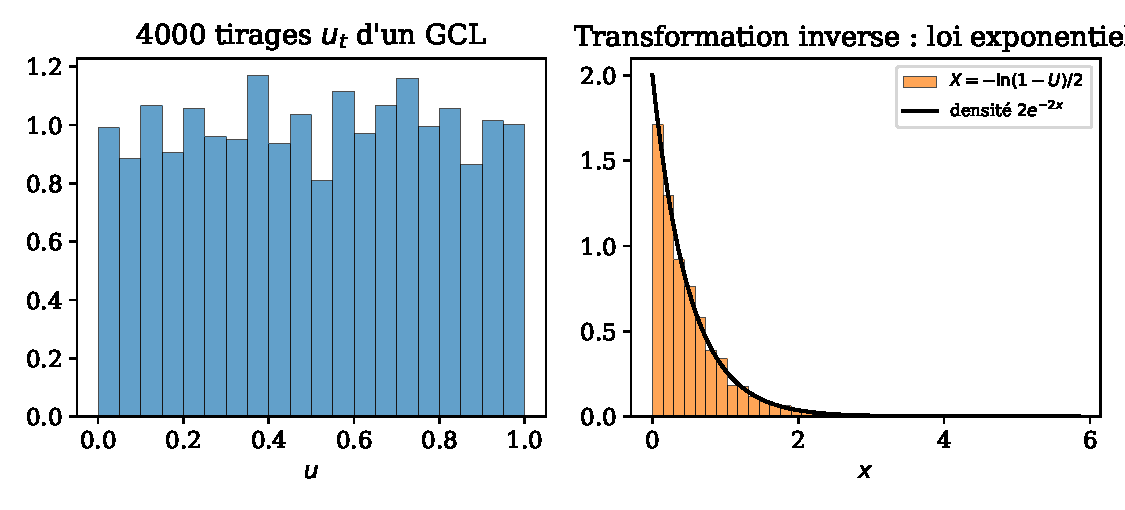
\includegraphics[width=0.85\textwidth]{figures/lcg.pdf}
\caption{Gauche : 4000 nombres produits par un GCL ($\lambda=1\,103\,515\,245$, $\alpha=12\,345$, $m=2^{31}$) ont l'air uniformes. Droite : transformés par $-\ln(1-u)/2$, ils suivent une loi exponentielle de paramètre 2.}
\end{figure}

\subsection{Les étapes de l'étude (cours p.~24)}
\begin{enumerate}
\item Fixer les « vraies » valeurs : $\beta_0$, $\beta_1$, $\sigma^2$.
\item Garder les $x_i$ \textbf{fixes} d'une réplication à l'autre (on étudie les propriétés conditionnelles à $\vX$, comme dans la théorie).
\item Pour $r=1,\dots,R$ : tirer de nouvelles erreurs $\epsilon_i^*$, construire $y_i^*=\beta_0+\beta_1x_i+\epsilon_i^*$, estimer par MCO, sauvegarder $b_{0r}^*$, $b_{1r}^*$ (et l'écart-type).
\item Analyser les $R$ estimations : moyenne (pour le biais), écart-type (pour la variance), histogramme (pour la loi).
\end{enumerate}
\begin{intuition}
La moyenne des $R$ estimations est elle-même une estimation de $\E[b_1]$, avec une erreur de simulation d'écart-type $\text{e.t.}(b_1)/\sqrt R$. Avec $R=10\,000$ et $\text{e.t.}(b_1)\approx0{,}034$, cette erreur est $\approx0{,}00034$ : un écart $|\bar b_1^*-\beta_1|$ de l'ordre de $0{,}0005$ (comme dans les résultats du cours) est donc tout à fait compatible avec l'absence de biais.
\end{intuition}

\subsection{Le code Stata commenté}
\begin{lstlisting}
capture drop _all                 // vide la mémoire
set seed 12345678                 // graine : résultats reproductibles
scalar beta0 = 1                  // vraies valeurs des paramètres
scalar beta1 = 1
scalar sigma = 1
global Nreps = 10000              // R : nombre de réplications
global Nobs  = 250                // n : taille de chaque échantillon
set obs $Nobs
gener double x = exp(rnormal(0,1)) // x log-normal, tiré UNE SEULE FOIS (fixe)
summarize x
scalar varbeta1 = sigma/( r(Var)*($Nobs-1) )  // Var(b1) = sigma^2 / somme (x-xbar)^2
scalar sdbeta1  = sqrt(varbeta1)              // vrai écart-type théorique
gener my = beta0 + beta1*x        // E[y|x], partie non aléatoire
gener epsilon = .                 // variables vides à remplir
gener sy = .
tempname simulate
postfile `simulate' b se using simresults, replace  // fichier de résultats
quietly {
 forvalues i = 1/$Nreps {
   replace epsilon = rnormal(0,sigma)  // nouvelles erreurs à chaque tour
   replace sy = my + epsilon           // nouvel échantillon y*
   reg sy x                            // MCO
   scalar b  = _b[x]                   // pente estimée
   scalar se = _se[x]                  // son écart-type estimé
   post `simulate' (b) (se)            // sauvegarde
 }
}
postclose `simulate'
use simresults, clear
summarize                         // moyenne et écart-type des 10 000 b et se
scalar list sdbeta1
histogram b, normal               // histogramme + densité normale superposée
\end{lstlisting}
\textbf{Remarques.} (i) \texttt{r(Var)*(\$Nobs-1)} $=\sum(x_i-\bar x)^2$ car la variance empirique de Stata divise par $n-1$. (ii) La formule utilise \texttt{sigma} là où il faudrait \texttt{sigma\^{}2} ; c'est sans conséquence ici puisque $\sigma=1$, mais le code serait faux pour $\sigma\neq1$. (iii) \texttt{rnormal(0,sigma)} prend l'\emph{écart-type} (pas la variance) en second argument, comme \texttt{rnorm} en R.

Le code R du cours fait exactement la même chose avec \texttt{set.seed}, \texttt{rnorm}, \texttt{lm} et une boucle \texttt{for} ; \texttt{summary(model)\$coef[2,1:2]} extrait la pente et son écart-type.

\subsection{Lecture des résultats}
\begin{center}
\begin{tabular}{@{}lccc@{}}
\toprule
& Stata (cours) & R (cours) & Python (notre réplication) \\
\midrule
Moyenne des $b_1^*$ & 0,999501 & 1,0002 & 0,99972 \\
Écart-type des $b_1^*$ & 0,03432 & -- & 0,02505 \\
Moyenne des e.t.\ estimés & 0,03441 & 0,03472 & 0,02521 \\
Vrai e.t.\ théorique & 0,03444 & 0,03475 & 0,02525 \\
Min / Max des $b_1^*$ & 0,876 / 1,120 & 0,863 / 1,120 & 0,899 / 1,104 \\
\bottomrule
\end{tabular}
\end{center}
(Les $x_i$ tirés diffèrent d'un logiciel à l'autre — même graine mais générateurs différents —, d'où des valeurs théoriques légèrement différentes ; dans notre tirage, les $x$ sont un peu plus dispersés, ce qui réduit la variance.)

Trois conclusions, toutes conformes à la théorie :
\begin{enumerate}
\item \textbf{Sans biais} : la moyenne des $b_1^*$ est à moins de $0{,}0005$ de la vraie valeur 1.
\item \textbf{Formule de variance correcte} : l'écart-type empirique des $b_1^*$ ($0{,}0343$) est égal à la valeur théorique $\sigma/\sqrt{\sum(x_i-\bar x)^2}$ ($0{,}0344$).
\item \textbf{Écart-type estimé sans biais (en pratique)} : la moyenne des e.t.\ calculés par \texttt{reg} ($0{,}0344$) retrouve la vraie valeur. Chaque e.t.\ individuel varie pourtant (de 0,028 à 0,041) : lui aussi est une variable aléatoire.
\end{enumerate}
Complément de notre réplication : l'intervalle de confiance à 95\,\% $b_1\pm t_{0{,}975;248}\,\text{e.t.}(b_1)$ contient la vraie valeur 1 dans \textbf{95,4\,\%} des 10\,000 échantillons — exactement ce qu'il doit faire.

\begin{figure}[h]
\centering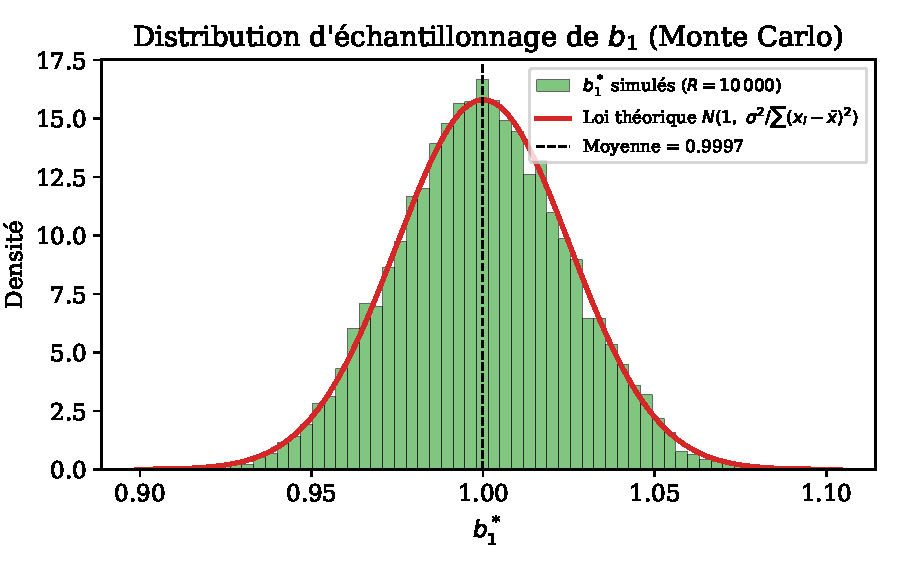
\includegraphics[width=0.72\textwidth]{figures/montecarlo.pdf}
\caption{Réplication de l'étude du cours ($n=250$, $R=10\,000$) : l'histogramme des pentes estimées coïncide avec la loi normale prédite par la théorie.}
\end{figure}

\subsection{Pourquoi l'histogramme est normal}
En bivarié, $b_1=\sum k_iy_i$ avec $k_i=(x_i-\bar x)/\sum(x_j-\bar x)^2$ [118]. En remplaçant $y_i$ : $b_1=\beta_1+\sum k_i\epsilon_i$ (car $\sum k_i=0$ et $\sum k_ix_i=1$). L'estimateur est donc une \textbf{combinaison linéaire des erreurs}. Une combinaison linéaire de variables normales indépendantes est normale, donc
\[
b_1\mid\vX\sim N\!\left(\beta_1,\ \frac{\sigma^2}{\sum(x_i-\bar x)^2}\right).
\]
Et en général, sous H5 : $\vb\mid\vX\sim N\big(\vbeta,\ \sigma^2\XtXi\big)$ — c'est la base des tests $t$ et $F$ du chapitre suivant.

\begin{intuition}[title={Et si les erreurs ne sont pas normales ?}]
Nous avons refait la simulation avec des erreurs très asymétriques (khi-deux à 1 degré de liberté, centrée et réduite). Résultat : moyenne des $b_1^*=0{,}99987$ (toujours sans biais, puisque H5 n'est pas nécessaire pour cela) et un histogramme toujours quasi normal, car $\sum k_i\epsilon_i$ est une somme de nombreux termes indépendants : c'est le \textbf{théorème central limite}, qui justifiera l'inférence « asymptotique » plus tard dans le cours.
\end{intuition}

% ======================= 12. COQUILLES =======================
\section{Coquilles et imprécisions relevées dans les notes}
Pour ne pas être déstabilisé en relisant les notes :
\begin{center}
\renewcommand{\arraystretch}{1.25}
\begin{tabular}{@{}p{2.3cm}p{6cm}p{6.5cm}@{}}
\toprule
Endroit & Écrit & Correct / remarque \\
\midrule
{[12]} & $-\vX'\vy+(\XtX)\vb=0$ & facteur 2 omis (sans conséquence) ; $\vb_0$ devient $\vb$ à l'optimum \\
§1.2, [16] & modèle en $\beta_0,\beta_1$, estimateurs $b_1,b_2$ & indices décalés : $b_1$ estime la constante, $b_2$ la pente \\
{[24]} & $\ve=\vX\vb-\vy$ & $\ve=\vy-\vX\vb$ (signe sans effet car $=0$) \\
{[31]} & $\hat{\bar y}_i=\bar y_i$ & pas d'indice $i$ : $\bar{\hat y}=\bar y$ \\
{[70]--[71]} & $(\vy-\vX_1\vb_0)(\vy-\vX_1\vb_0)$ & manque un prime : $(\vy-\vX_1\vb_0)'(\vy-\vX_1\vb_0)$ \\
{[75]} & $\vX_2$ & $\vx_2$ (une seule variable ajoutée) \\
§2.4.1 & SCE puis SSE & même quantité (somme des carrés des résidus) \\
{[81]} & $\E[(\vb-\E(\vb))\dots]$ & correct ; on remplace $\E(\vb)$ par $\vbeta$ grâce à l'absence de biais \\
§4, [87]--[90] & $\C\vX=\I_n$, $\D\vX+\I_n=\I_n$ & $\I_K$ (matrice $K\times K$) \\
{[93]} & $\Var(\vb\mid\vX)\le\Var(\vb^*\mid\vX)$ & au sens matriciel : la différence est semi-définie positive \\
{[106]--[107]} & parenthèses en trop & $\E(\ve'\ve\mid\vX)=\sigma^2(n-K)$, $\E(s^2\mid\vX)=\sigma^2$ \\
Code Stata & \texttt{sigma/(r(Var)*(\$Nobs-1))} & devrait être \texttt{sigma\^{}2/(\dots)} ; identique ici car $\sigma=1$ \\
p.~27 & « la variance de $b_1$ est sd$(b_1)=\dots$ » & c'est l'écart-type (racine de la variance) \\
\bottomrule
\end{tabular}
\end{center}

% ======================= 13. FICHE =======================
\section{Fiche de révision}
\begin{tcolorbox}[colback=white,colframe=NavyBlue,title=Les formules essentielles]
\small\begin{align*}
\text{Estimateur :}\ & \vb=\XtXi\vX'\vy \quad(\text{bivarié : } b_2=\tfrac{\sum(x_i-\bar x)(y_i-\bar y)}{\sum(x_i-\bar x)^2},\ b_1=\bar y-b_2\bar x)\\
\text{Équations normales :}\ & \vX'\ve=\mathbf 0\quad(\text{avec constante : }\textstyle\sum e_i=0,\ \bar y=\bar{\vx}'\vb,\ \bar{\hat y}=\bar y)\\
\text{Projections :}\ & \Pm=\vX\XtXi\vX',\ \Mm=\I-\Pm;\ \Mm\vX=\mathbf 0,\ \Pm\vX=\vX\\
\text{FWL :}\ & \vb_2=(\vX_2'\Mm_1\vX_2)^{-1}\vX_2'\Mm_1\vy\\
\text{Décomposition :}\ & \text{SCT}=\text{SCR}+\text{SCE},\quad R^2=1-\text{SCE}/\text{SCT},\quad \bar R^2=1-\tfrac{n-1}{n-K}(1-R^2)\\
\text{Ajout d'une variable :}\ & \text{SCE}_2=\text{SCE}_1-\tilde b_2^2\,\vx_2'\Mm_1\vx_2\le\text{SCE}_1\\
\text{Sans biais (H1--H3) :}\ & \vb=\vbeta+\XtXi\vX'\veps,\quad \E[\vb\mid\vX]=\vbeta\\
\text{Variance (H4) :}\ & \Var(\vb\mid\vX)=\sigma^2\XtXi\\
\text{Gauss-Markov :}\ & \Var(\vb^*\mid\vX)=\Var(\vb\mid\vX)+\sigma^2\D\D'\\
\text{Estimation de }\sigma^2\text{ :}\ & s^2=\ve'\ve/(n-K),\quad \E[\ve'\ve]=\sigma^2\tr(\Mm)=\sigma^2(n-K)\\
\text{Normalité (H5) :}\ & \vb\mid\vX\sim N(\vbeta,\sigma^2\XtXi)
\end{align*}
\end{tcolorbox}

\textbf{Les 8 idées à comprendre (pas seulement à mémoriser)}
\begin{enumerate}[nosep]
\item Les MCO minimisent une somme de carrés ; la solution est la projection orthogonale de $\vy$ sur l'espace des $\vX$.
\item Les résidus sont orthogonaux aux régresseurs \emph{par construction} : cela ne prouve rien sur l'exogénéité.
\item Propriétés numériques = toujours vraies ; propriétés statistiques = dépendent des hypothèses.
\item FWL = « toutes choses égales par ailleurs » en langage matriciel.
\item Le $R^2$ ne baisse jamais quand on ajoute une variable : il ne sert pas à choisir un modèle.
\item Sans biais repose sur $\E[\veps\mid\vX]=\mathbf0$ ; la formule de variance sur $\sigma^2\I$.
\item Gauss-Markov : parmi les estimateurs linéaires sans biais, les MCO ont la plus petite variance (pas besoin de normalité).
\item On divise par $n-K$ car $K$ degrés de liberté sont « consommés » par l'estimation de $\vb$.
\end{enumerate}

% ======================= 14. EXERCICES =======================
\section{Exercices corrigés}

\textbf{Exercice 1.} Montrer que dans une régression sur une constante seule ($\vX=\vi$), $b=\bar y$ et $s^2$ est la variance empirique usuelle.

\emph{Corrigé.} $\vi'\vi=n$ et $\vi'\vy=\sum y_i$, donc $b=\frac1n\sum y_i=\bar y$. Les résidus sont $y_i-\bar y$ et $K=1$, d'où $s^2=\frac{1}{n-1}\sum(y_i-\bar y)^2$. On retrouve le « $n-1$ » du cours de statistique comme cas particulier de $n-K$.

\medskip
\textbf{Exercice 2.} On multiplie la variable $x$ par 100 (on passe de dollars en cents). Que deviennent $b_2$, $b_1$, les résidus et le $R^2$ ?

\emph{Corrigé.} $\sum(100x_i-100\bar x)(y_i-\bar y)/\sum(100x_i-100\bar x)^2=b_2/100$. $b_1=\bar y-(b_2/100)(100\bar x)$ est inchangé. Les valeurs prédites, donc les résidus et le $R^2$, sont inchangés : $\Pm$ ne dépend que de l'espace engendré par les colonnes de $\vX$, qui ne change pas quand on multiplie une colonne par une constante.

\medskip
\textbf{Exercice 3.} Montrer que $\tr(\Pm)=K$ et en déduire $\sum_i p_{ii}=K$ (la moyenne des leviers est $K/n$).

\emph{Corrigé.} $\tr(\vX\XtXi\vX')=\tr(\XtXi\XtX)=\tr(\I_K)=K$. La trace étant la somme des éléments diagonaux, $\sum p_{ii}=K$.

\medskip
\textbf{Exercice 4.} Avec l'exemple numérique ($x=1,\dots,5$), on considère l'estimateur « premier et dernier point » $b_2^*=(y_5-y_1)/(x_5-x_1)$. (a) Montrer qu'il est linéaire et sans biais. (b) Comparer sa variance à celle des MCO.

\emph{Corrigé.} (a) $b_2^*=(y_5-y_1)/4$ est linéaire en $\vy$. $\E[b_2^*]=\frac{(\beta_1+5\beta_2)-(\beta_1+\beta_2)}{4}=\beta_2$ : sans biais. (b) $\Var(b_2^*)=\frac{2\sigma^2}{16}=0{,}125\,\sigma^2$, contre $\Var(b_2)=\sigma^2/\sum(x_i-\bar x)^2=\sigma^2/10=0{,}1\,\sigma^2$. Les MCO sont plus précis, comme le garantit Gauss-Markov.

\medskip
\textbf{Exercice 5.} Pourquoi ne peut-on pas utiliser $\frac1n\sum e_i^2$ pour estimer $\sigma^2$ ? Calculer son biais.

\emph{Corrigé.} $\E[\frac1n\ve'\ve]=\frac{n-K}{n}\sigma^2<\sigma^2$ : il sous-estime $\sigma^2$ d'un facteur $(n-K)/n$. Le biais, $-\frac Kn\sigma^2$, disparaît quand $n\to\infty$ (l'estimateur est convergent), mais peut être important en petit échantillon (dans notre exemple, $n=5$, $K=2$ : 40\,\% de sous-estimation).

\medskip
\textbf{Exercice 6.} Vrai ou faux : « Comme $\sum x_ie_i=0$ dans ma régression, l'hypothèse $\E[\epsilon\mid x]=0$ est vérifiée. »

\emph{Corrigé.} Faux. $\sum x_ie_i=0$ est une propriété numérique vraie pour n'importe quelles données, même si $x$ est endogène. L'exogénéité porte sur les \emph{erreurs} inobservables, pas sur les résidus ; elle se justifie par un argument économique (ou un dispositif expérimental), pas par ce calcul.

\medskip
\textbf{Exercice 7 (Monte Carlo).} Dans l'étude du cours, que se passerait-il si l'on générait des erreurs avec $\E[\epsilon_i\mid x_i]=0{,}2\,x_i$ ?

\emph{Corrigé.} Alors $y_i=1+x_i+\epsilon_i$ avec $\epsilon_i=0{,}2x_i+u_i$, soit $y_i=1+1{,}2x_i+u_i$. Les MCO estimeraient en moyenne $1{,}2$ au lieu de 1 : biais de $0{,}2$, visible comme un décalage de l'histogramme, qui ne disparaîtrait pas en augmentant $R$ ou $n$. C'est une illustration de la violation de H3.

% ======================= REFERENCES =======================
\section*{Références et sources consultées}
\addcontentsline{toc}{section}{Références et sources consultées}
\begin{itemize}[leftmargin=*]
\item W. H. Greene, \emph{Econometric Analysis}, Pearson (ch.~3 : MCO ; ch.~4 : propriétés statistiques ; ch.~15.5 : Monte Carlo).
\item A.-M. Legendre (1805), \emph{Nouvelles méthodes pour la détermination des orbites des comètes}, appendice « Sur la méthode des moindres quarrés ». Présentation : \url{http://www.bibnum.education.fr/mathematiques/algebre/legendre-et-la-methode-des-moindres-carres}
\item « Méthode des moindres carrés », Wikipédia : \url{https://fr.wikipedia.org/wiki/M\%C3\%A9thode_des_moindres_carr\%C3\%A9s}
\item R. Frisch et F. V. Waugh (1933), « Partial Time Regressions as Compared with Individual Trends », \emph{Econometrica} 1(4). M. C. Lovell (1963), « Seasonal Adjustment of Economic Time Series and Multiple Regression Analysis », \emph{JASA} 58.
\item D. Basu (2023), « The Yule-Frisch-Waugh-Lovell Theorem », \url{https://arxiv.org/abs/2307.00369}
\item P. Ding (2021), « The Frisch--Waugh--Lovell theorem for standard errors », \emph{Statistics \& Probability Letters}.
\item « Gauss--Markov theorem », Wikipedia : \url{https://en.wikipedia.org/wiki/Gauss\%E2\%80\%93Markov_theorem} ; A. C. Aitken (1935), « On Least Squares and Linear Combinations of Observations », \emph{Proc. Royal Soc. Edinburgh} 55.
\item B. E. Hansen (2022), « A Modern Gauss-Markov Theorem », \emph{Econometrica} 90(3) : \url{https://users.ssc.wisc.edu/~behansen/papers/gauss.pdf}
\item H. Theil (1961), \emph{Economic Forecasts and Policy} (introduction du $R^2$ ajusté).
\item « Linear congruential generator » et « RANDU », Wikipedia : \url{https://en.wikipedia.org/wiki/Linear_congruential_generator}, \url{https://en.wikipedia.org/wiki/RANDU} ; G. Marsaglia (1968), « Random numbers fall mainly in the planes », \emph{PNAS} 61.
\item N. Metropolis et S. Ulam (1949), « The Monte Carlo Method », \emph{JASA} 44.
\end{itemize}
\textit{Les figures et la réplication de Monte Carlo ont été produites avec Python (NumPy, Matplotlib) ; le script \texttt{figures.py} est fourni avec ce document.}

\end{document}
